\documentclass[a4paper]{article}
\usepackage[utf8]{inputenc}
\usepackage[T1]{fontenc}
\usepackage{graphicx}
\usepackage{float}
\setkeys{Gin}{width=\linewidth, keepaspectratio}

\begin{document}

\title{Rapport projet couverture de graphe}
\author{Rémi Pérenne et Viktoriia Skrypnyk}
\maketitle

Q3.1 :
L'algorithme glouton n'est pas optimale car pour le graphe ci-dessous, il trouve \{0,1,2,3\} comme couverture alors que la couverture minimale est \{1,2,3\}. Il n'est donc pas 1.3-approché.

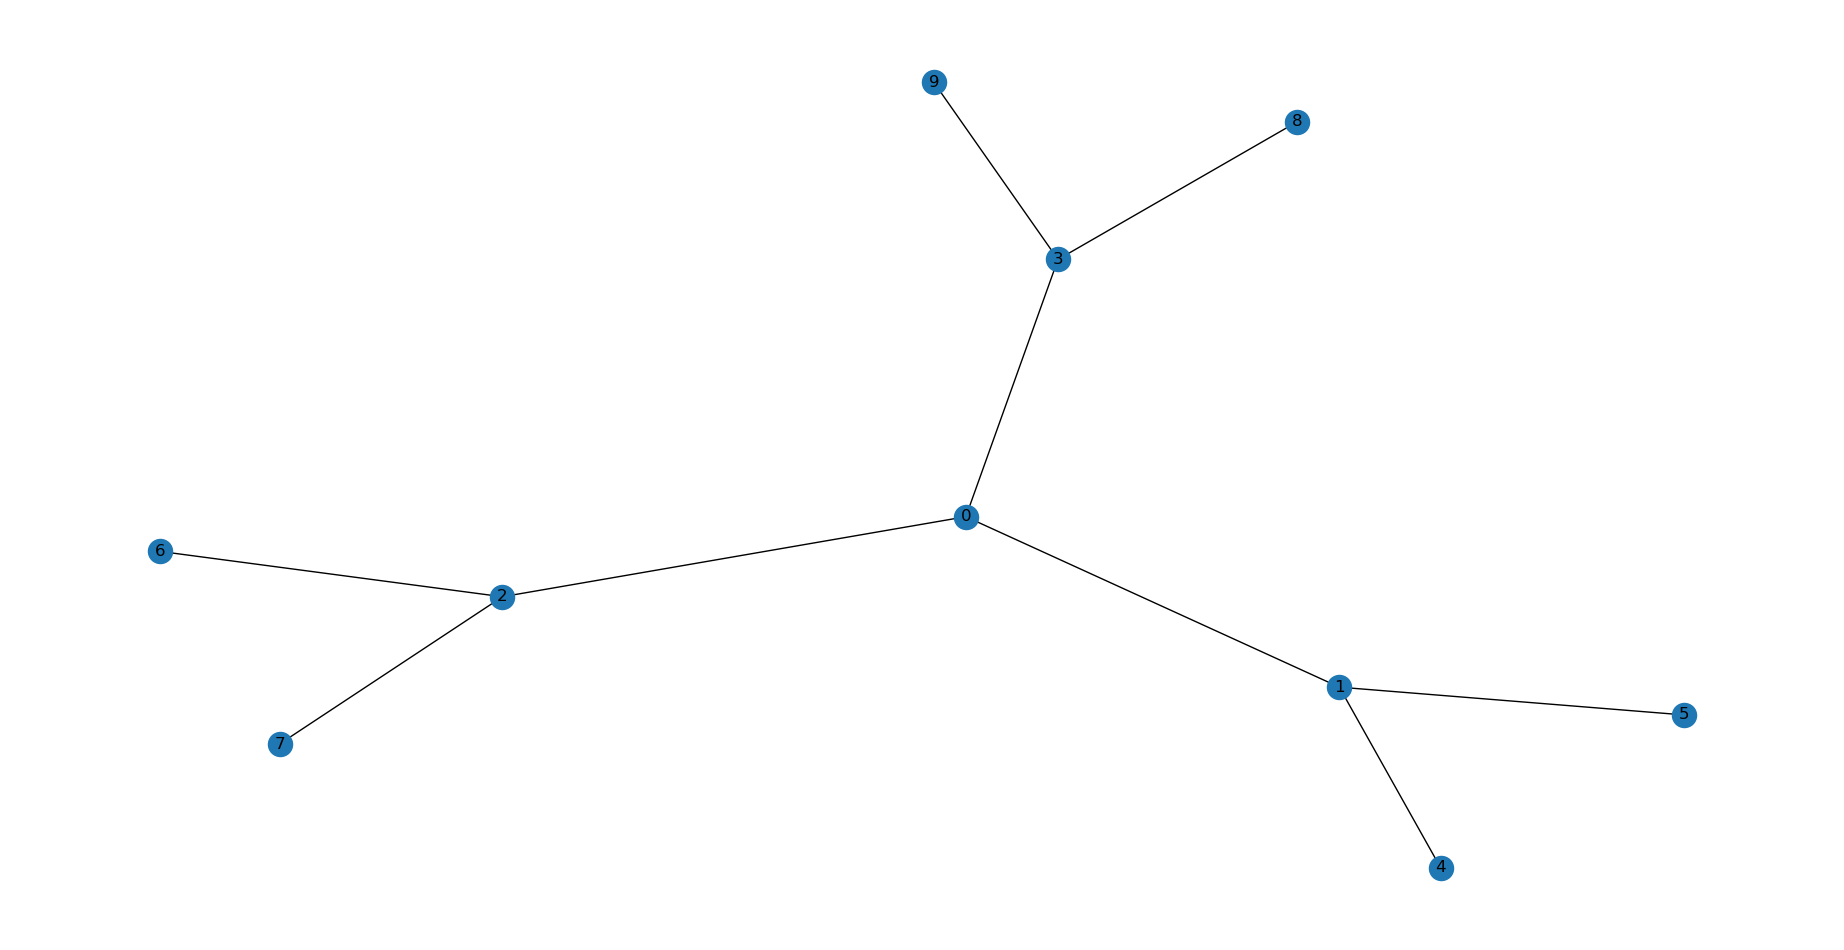
\includegraphics{"./graphe_q31.png"}

Q3.2 :
Voilà des graphiques permettant de comparer les 2 méthodes d'approximation. On peut voir que l'algorithme glouton donne sur les exemples des resultats similaire à la couverture minimale (calculée à l'aide d'un algorithme tiré des questions suivantes). L'algorithme de couplage quand à lui donne effectivement des ensembles d'aretes dont le cardinal est au plus deux fois le cardinal d'une couverture minimale. On voit aussi que l'algorithme glouton prend bien plus de temps que l'algorithme de couplage pour s'executer. Ces observations sont vraies pour toutes les valeurs de $p$.

\includegraphics{"./q32a.png"}
\includegraphics{"./q32b.png"}

Q3.3 :
Soit $n$ un entier. Considérons le graphe $G_n$ dont les sommets sont partitionnés entre $A_n$ qui contient $n$ sommets et les $B_n^k$ définis par $|B_n^k| = \lfloor n/k \rfloor $ et chaque sommets de $B_n^k$ a $k$ voisins dans $A_n$ et deux sommets de $B_n^k$ n'ont pas de voisins commun dans $A_n$. On vérifie que $A_n$ est une couverture du graphe. Mais il est possible que l'algorithme glouton prennent successivement tout les sommets de $B_n^n$ puis les sommets de $B_n^{n-1}$ et ainsi de suite jusqu'à prendre tout les sommets de $B_n^1$. Ce qui fait de l'ordre de $nlogn$ sommets (séries harmonique). Ainsi en faisant tendre $n$ vers l'infinie on obtient que l'algorithme glouton n'est pas r-approché pour tout r.
\\

Q4.1.2 :
Voilà des graphiques permettant de tester le temps ainsi que le nombre de noeuds générés par l'algorithme de branchement. On constate effectivement une évolution exponentiel du nombre de noeuds et du temps pris pour executer la fonction en fonction du nombre de noeuds $n$ dans le graphe.

\includegraphics{"./q412a.png"}
\includegraphics{"./q412b.png"}

Q4.2.1 : Pour la borne $b_1$, on sait qu'il y a $m$ aretes et que lorsque l'on prend un sommet on prend au plus $\Delta$ aretes ainsi il faut prendre au moins $ \lceil \frac{m}{\Delta} \rceil $ sommets pour prendre toutes les aretes (la partie entière suérieure est là car on ne peut prendre qu'un nombre entier d'aretes...)

Pour la borne $b_2$, il faut prendre une des deux extremités de chaque arete du couplage dans une couverture. Mais les aretes du couplage ne partagent aucun sommet il faut donc prendre au moins $|M|$ sommets.

Pour la borne $b_3$ on note qu'il y a $|C|$ sommets dans la couverture et $n-|C|$ sommets qui ne sont pas dans la couverture. Ainsi,  $m \leq \frac{|C|(|C|-1)}{2} + (n-|C|)|C|$ (en effet, chaque sommet de $C$ est connecté à au plus tout les autres sommets du graphe et les sommets qui ne sont pas dans la couverture ne peuvent pas être lié entre eux sinon il y aurait des aretes non couvertes... la formule s'obtient ensuite par combinatoire). Les racines de $|C| + (1-2n)|C| + 2m = 0$ sont $|C| = \frac{2n - 1 \pm \sqrt{(2n-1)^2 - 8m}}{2}$ donc $m \leq \frac{|C|(|C|-1)}{2} + (n-|C|)|C| \iff |C| \in [\frac{2n - 1 - \sqrt{(2n-1)^2 - 8m}}{2};\frac{2n - 1 + \sqrt{(2n-1)^2 - 8m}}{2}]$ donc $|C| \leq \frac{2n - 1 + \sqrt{(2n-1)^2 - 8m}}{2}$ ce qui est le résultat attendu. \\

Q4.2.2 : 
Voilà des graphiques permettant de tester le temps ainsi que le nombre de noeuds générés par l'algorithme de branchement avec bornes. On constate effectivement une évolution exponentiel du nombre de noeuds et du temps pris pour executer la fonction en fonction du nombre de noeuds $n$ dans le graphe mais c'est bien plus rapide que sans les bornes !

\includegraphics{"./q422a.png"}
\includegraphics{"./q422b.png"}

Q4.2.3 : 
Voilà un graphique permettant de tester le temps d'execution avec l'algorithme glouton pour sélectionner quelle branche on visite en premier. On constate que l'algorithme glouton est trop long à executer par rapport au temps qu'il fait gagner... Cette méthode n'est donc pas rentable.

\includegraphics{"./q423a.png"}
\includegraphics{"./q423b.png"}

C'est encore pire si on n'utilise que le glouton sans la borne inf:

\includegraphics{"./q423c.png"}
\includegraphics{"./q423d.png"}

Q4.3.1 : 
Le branchement amélioré fait gagner beaucoup de temps et de noeuds visités !

\includegraphics{"./q431a.png"}
\includegraphics{"./q431b.png"}

Q4.3.1 : 
C'est déjà ce que l'on fait depuis le début sans avoir vu cette question.

Q4.3.3 :
Soit $G$ un graphe et $C$ un couverture minimale de $G$ ainsi que $s$ un sommet de degré 1 de $G$. Si $s \in C$, notons $v$ l'unique voisin de $s$ qui n'est pas dans $C$ (il existe sinon $C\textbackslash\{s\}$ est une couverture de taille strictement inférieure à $C$). Alors $(C\textbackslash\{s\}) \cup \{v\}$ est une couverture de $G$ qui ne contient pas $s$. Ainsi pour tout sommet $s$ de degré 1, il existe une couverture qui ne contient pas $s$. \\
\includegraphics{"./q433a.png"}
\includegraphics{"./q433b.png"}
On observe que cette heuristique fait encore gagner du temps et réduit encore le nombre de noeuds visités. \\

Q4.4.1 : 
Voilà des graphiques permettant de comparer les rapports d'approximation de l'algorithme glouton et de l'algorithme de couplage. Le pire rapport pour l'algorithme de couplage est 1,8 et le pire rapport pour l'algorithme glouton est 1,1. On observe aussi que l'algorithme de couplage semble être meilleur lorsque n augmente.

\includegraphics{"./q441a.png"}
\includegraphics{"./q441b.png"}

\end{document}
